\documentclass[11pt]{exam}

\oddsidemargin=0.25truein \evensidemargin=0.25truein
\topmargin=-0.5truein \textwidth=6.0truein \textheight=8.75truein

%\RequirePackage{graphicx}
\usepackage{comment}
\usepackage{verbatim}
\usepackage{booktabs}
\usepackage{graphicx}
\usepackage{hyperref}
\urlstyle{rm}   % change fonts for url's (from Chad Jones)
\hypersetup{
    colorlinks=true,        % kills boxes
    allcolors=blue,
    pdfsubject={ECON-UB233, Macroeconomic foundations for asset pricing},
    pdfauthor={Dave Backus @ NYU},
    pdfstartview={FitH},
    pdfpagemode={UseNone},
%    pdfnewwindow=true,      % links in new window
%    linkcolor=blue,         % color of internal links
%    citecolor=blue,         % color of links to bibliography
%    filecolor=blue,         % color of file links
%    urlcolor=blue           % color of external links
% see:  http://www.tug.org/applications/hyperref/manual.html
}

\renewcommand{\thefootnote}{\fnsymbol{footnote}}
\newcommand{\var}{\mbox{\it Var\/}}

%\printanswers

% document starts here
\begin{document}
\parskip=\bigskipamount
\parindent=0.0in
\thispagestyle{empty}
{\large ECON-UB 233 \hfill Dave Backus @ NYU}

\bigskip\bigskip
%\centerline{\Large \bf Lab Report \#7:  Stochastic Processes}
\centerline{\Large \bf Lab Report \#7:  Dynamics in Theory and Data}
\centerline{(Started: April 11, 2012; Revised: \today)}

\bigskip
{\it Due at the start of class.
You may speak to others, but whatever you hand in should be your own work.}

\begin{questions}

\begin{solution}
Answers follow.  See Matlab code at the end for calculations.
\end{solution}

%-----------------------------------------------------------------------
\question (dynamics of interest rates)
We'll look at the autocorrelations of interest rates to get a sense
of their dynamics.
The first step is to download some data from the Fed.
Go to

\url{http://www.federalreserve.gov/releases/h15/data.htm}

and download monthly data for Treasury constant maturities,
specifically the 3-month and 10-year maturities,
for the period 1985 to present.
Read them into Matlab and:


\begin{parts}
\part Compute the mean, standard deviation,
and autocorrelation function (acf) for the 1-month
interest rate.
(You may recall that we used the program {\tt acf.m} for the latter
in class.  It's our program, not part of Matlab, although Matlab's
Econometrics Toolbox has a similar function.
It works on time series objects, which is something I'd prefer to avoid for now.
But by all means do whatever you wish.)

\part Describe the acf for an AR(1):
\begin{eqnarray*}
    x_t &=& (1-\varphi) \mu + \varphi x_{t-1} + \theta w_t ,
\end{eqnarray*}
where $ \{ w_t \} \sim \mbox{NID}(0,1)$.
How do the acf's compare for the data and a suitably estimated AR(1)?
\part Compute the mean, standard deviation,
autocorrelation function (acf) for the 10-year interest rate.
How do they compare to the 1-month rate?
\end{parts}

\begin{solution}
\begin{enumerate}
\item [(a,c)]
The relevant statistics are

\begin{center}
\begin{tabular}{lccc}
\toprule
        &  Mean & Std Dev & Autocorr \\
\midrule
3-month  &   4.14 & 2.45 & 0.988  \\
10-year  &   5.94 & 2.05 & 0.976  \\
\bottomrule
\end{tabular}
\end{center}

They reflect some standard features of interest rates, including:
(i)~rates increase with maturity, on average;
(ii)~standard deviations decline with maturity;
and (iii)~all of them are very persistent.
Which is the point of the exercise.

We can see more of the autocorrelation functions in this figure:
\begin{center}
%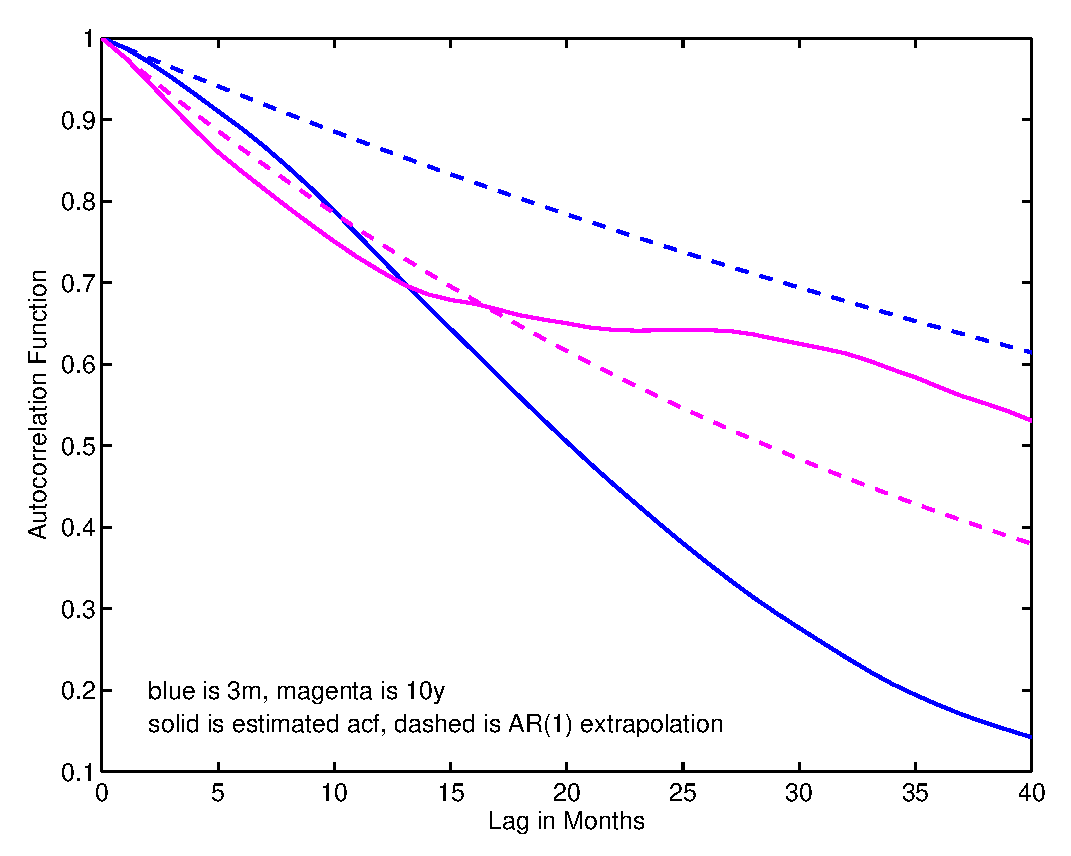
\includegraphics[width=4in]{../Matlab/hw7_q1ab.eps}
\end{center}

\item[(b)] With an AR(1), the autocorrelation has the form
$\rho(k) = \varphi^k$:  it declines geometrically.
If we set $\varphi = \rho(1)$, we can compute
estimated acf's corresponding to AR(1)s.
They're plotted as the dashed lines above.
You can see they're somewhat different from the AR(1).
Whether this represents sampling variability of some more
basic difference between the data and the AR(1) model isn't clear.


\end{enumerate}
\end{solution}

%-----------------------------------------------------------------------
\question (two-state Markov chain)
We can get a sense of how Markov chains work with a two-state example.
A two-state chain is characterized by a 2 by 2 transition matrix $P$.
Because the rows sum to one, $P$ has (essentially) two parameters.
A convenient parameterization is
\begin{eqnarray}
    P &=& (1-\varphi)
        \left[
        \begin{array}{cc}
        \omega & 1-\omega \\ \omega & 1-\omega
        \end{array}
        \right]
        + \varphi
        \left[
        \begin{array}{cc}
        1  & 0  \\  0  & 1
        \end{array}
        \right] ,
        \label{eq:p-simple}
\end{eqnarray}
where the two parameters are $\omega$ and $\varphi$.

\begin{parts}
\part Under what conditions on $(\omega, \varphi)$ is $P$ a legitimate
transition matrix?
\part What are the two-period transitions $P^2$?
You can either do this by hand or get Matlab to do it.  Either way,
the key is to arrange the terms into a form similar to (\ref{eq:p-simple}).
\part What about the $k$-period transitions?
\part What happens as we continue to increase $k$?
What is the equilibrium distribution?
\part (extra credit) What are the eigenvalues of $P$?
\end{parts}

\begin{solution}
This is the simplest possible Markov chain,
but it illustrates more general properties quite nicely.
\begin{enumerate}
\item [(a)] The probabilities have to be between zero and one,
which gives us these inequalities:
\begin{eqnarray*}
    0 &\leq& (1-\varphi) \omega + \varphi \;\;\leq\;\; 1 \\
    0 &\leq& (1-\varphi) (1-\omega) \;\;\leq\;\; 1 \\
    0 &\leq& (1-\varphi) \omega \;\;\leq\;\; 1 \\
    0 &\leq& (1-\varphi) (1-\omega) + \varphi \;\;\leq\;\; 1 .
\end{eqnarray*}
That's sufficient for your answer.
If you'd like to go further, here's how it works.
The second and third inequalities imply (add them together)
$ - 1 \leq \varphi \leq 1 $.
The first and fourth imply $ 0 \leq \omega \leq 1$.
That's not quite sufficient though.
The second and third imply (directly, divide by $1-\varphi$)
\begin{eqnarray*}
        - \varphi /(1-\varphi) \;\;\leq\;\; \omega \;\;\leq\;\; 1/(1-\varphi),
\end{eqnarray*}
a joint restriction on $\omega$ and $\varphi$.
If $\varphi \geq 0$ this is irrelevant,
it's less restrictive than our earlier condition on $\omega$.
But if $\varphi < 0$, it limits the range of $\omega$.
For example, if $\varphi = -1/2$,
then $ 1/3 \leq \omega \leq 2/3$.



\item [(b,c)] The $k$-period transitions have the form
\begin{eqnarray*}
    P &=& (1-\varphi^k)
        \left[
        \begin{array}{cc}
        \omega & 1-\omega \\ \omega & 1-\omega
        \end{array}
        \right]
        + \varphi^k
        \left[
        \begin{array}{cc}
        1  & 0  \\  0  & 1
        \end{array}
        \right] .
\end{eqnarray*}

\item [(d)]
Eventually $\varphi^k \rightarrow 0$ and $P$ converges to the
first matrix.
The equilibrium distribution is evidently $(\omega, 1-\omega)$.

\item [(e)]
If you're comfortable with linear algebra, you might notice that
$P$ has eigenvalues of 1 and $\varphi$.
The first is a feature of all Markov chains:
since the rows sum to one, there's an eigenvalue of one.
The second tells you how fast you converge to the equilibrium
distribution.

\end{enumerate}
\end{solution}


%-----------------------------------------------------------------------
\question (state-space representations)
State-space models have a similar mathematical structure
in the sense that dynamics follow from powers of a matrix.
The canonical version is
\begin{eqnarray}
    x_{t+1} &=& A x_t + B w_{t+1} .
    \label{eq:state-space}
\end{eqnarray}
Here $x$ is a vector, $w \sim \mathcal{N}(0,I)$
is also a vector (of possibly different dimension),
and $(A,B)$ are matrices.

\begin{parts}
\part Consider the ARMA(1,1):
\begin{eqnarray*}
    y_t &=& \varphi_1 y_{t-1} + \theta_0 w_t + \theta_1 w_{t-1} .
\end{eqnarray*}
Show that this can be expressed in the same form as (\ref{eq:state-space}).
\part Ditto for the ARMA(2,1):
\begin{eqnarray*}
    y_t &=& \varphi_1 y_{t-1} + \varphi_2 y_{t-2} + \theta_0 w_t + \theta_1 w_{t-1} .
\end{eqnarray*}
\part (extra credit) For the general model (\ref{eq:state-space}),
what is the distribution of $x_{t+2}$ given $x_t$?
\part (extra credit) Ditto for $x_{t+k}$.
Under what conditions does this converge as $k$ gets large?

\end{parts}

\begin{solution}
This course is designed to use linear algebra sparingly.
Nevertheless, in this case you might want to know
that what seem like relatively complex models can often
be written simply in matrix form.
In that case, we're dealing with essentially higher-dimensional
analogs of an AR(1).
That makes programming and insight much easier.
We won't use it in this class,
but keep in mind that we can easily extend most of our models
to higher dimensions with little difference in the analysis.
If this line of thought doesn't work for you,
just ignore what follows, it won't come up again.

\begin{parts}
\part The ARMA(1,1) can be written
\begin{eqnarray*}
    \left[
    \begin{array}{c}
    y_{t+1} \\ w_{t+1}
    \end{array}
    \right]
    &=&
    \left[
    \begin{array}{cc}
    \varphi_1 & \theta_1 \\ 0 & 0
    \end{array}
    \right]
    \left[
    \begin{array}{c}
    y_{t} \\ w_{t}
    \end{array}
    \right]
    +
    \left[
    \begin{array}{c}
    \theta_0 \\ 1
    \end{array}
    \right]
    [w_{t+1} ] ,
\end{eqnarray*}
which you should recognize from the notes on stochastic processes.

\part The ARMA(2,1) becomes
\begin{eqnarray*}
    \left[
    \begin{array}{c}
    y_{t+1} \\ y_t \\ w_{t+1}
    \end{array}
    \right]
    &=&
    \left[
    \begin{array}{ccc}
    \varphi_1 & \varphi_2 & \theta_1 \\ 1 & 0 & 0 \\ 0 & 0 & 0
    \end{array}
    \right]
    \left[
    \begin{array}{c}
    y_{t} \\ y_{t-1} \\ w_{t}
    \end{array}
    \right]
    +
    \left[
    \begin{array}{c}
    \theta_0 \\ 0 \\ 1
    \end{array}
    \right]
    [w_{t+1} ] .
\end{eqnarray*}

\part Now we can put the AR(1) structure to work.  After substituting,
\begin{eqnarray*}
    x_{t+2} &=& A^2 x_t + B w_{t+2} + A B w_{t+1} .
\end{eqnarray*}
The first term ($A^2 x_t$) is the conditional mean.
The others generate variance.  It goes beyond this course,
but for a vector like $w_t$ the variance is a matrix,
with variances on the diagonal and covariances otherwise.
If that's confusing, just skip it.

If not, we write the variance matrix as $E (w_t w_t^\top)$,
where $^\top$ is a brute force way to write the transpose.
In our case, we assumed the variance matrix for $w_t$ is $I$,
with ones on the diagonal and zeros off.

What's the variance matrix for $x_{t+2}$?
It's defined by
\begin{eqnarray*}
        \mbox{Var}_t (x_{t+2}) &=&
        E_t \left[ (x_{t+2} - A x_t) (x_{t+2} - A x_t)^\top \right] \\
                &=&
                E_t \left[ (B w_{t+2} + A B w_{t+1}) (B w_{t+2} + A B w_{t+1})^\top \right] \\
        &=& B B^\top + A B B^\top A^\top .
\end{eqnarray*}

\part Same idea repeated:
\begin{eqnarray*}
        \mbox{Var}_t (x_{t+k}) &=&
         B B^\top + A B B^\top A^\top + A^2 B B^\top (A^2)^\top
                + \cdots + A^{k-1} B B^\top (A^{k-1})^\top .
\end{eqnarray*}
As $k$ gets large, we get more terms.
It converges, though, if the terms shrink fast enough,
which requires powers of $A$ to shrink.
If you're familiar with linear algebra,
you need the eigenvalues of $A$ to be less than one in
absolute value.

\end{parts}
\end{solution}

\end{questions}

\vfill \centerline{\it \copyright \ \number\year \
NYU Stern School of Business}

\pagebreak
Matlab program:
\verbatiminput{../Matlab/hw7_s12.m}

\end{document}


%  EXTRA STUFF


